\section{レーザー測定のセットアップ}

以下の 図\ref{fg:Laser_setup} にこの実験の測定のセットアップを示す。
赤外線パルスレーザーをセンサーに入射し、センサーからの信号をアンプボードで増幅を行い、オシロスコープへと信号を送る。
トリガーはレーザー本体からオシロスコープへ送っている。トリガーと信号を受け取ったオシロスコープはPCへとデータを送り出す。
使用するオシロスコープは、TELEDYNE LECROY 社の WaveRunner 8000HD 8チャンネル 高分解能オシロスコープで、サンプリングレートは最大10GS/sである。
センサーとアンプボードの下には、アンプボードの発熱による温度上昇を抑えるために、
15${}^\circ$Cに設定されたチラーユニットと20${}^\circ$Cに設定されたペルチェ素子を設置した。
この装置の冷却が銅板に伝わり、空冷によってセンサーの温度上昇を抑えている。
また、センサーに光が入ると、センサーの暗電流が大きくなってしまうため、測定のセットアップを遮光するためにボックスの中に設置した。
一度の測定のイベント数は65535イベントでこのイベント数はオシロスコープの一回の測定による上限値である。

\begin{figure}[h]
    \centering
    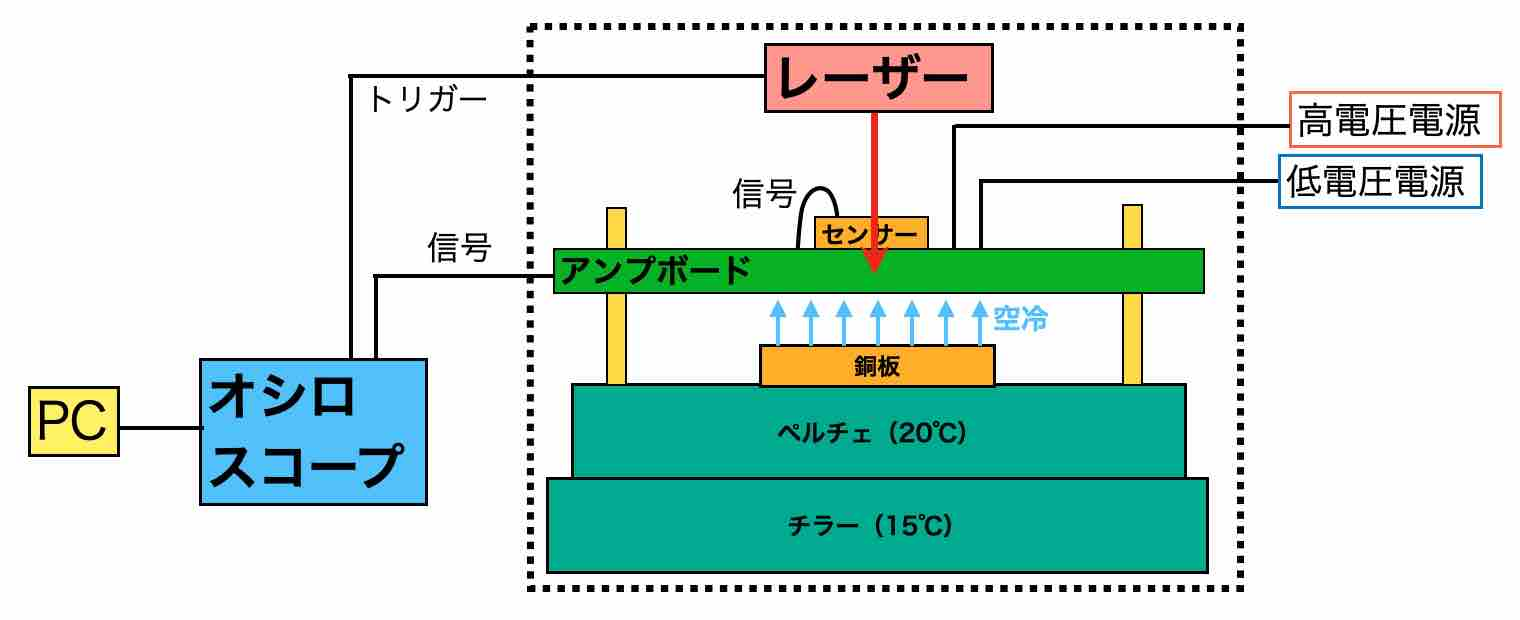
\includegraphics[width=14cm]{fig/ch4/Laser_setup.jpg}
    \caption[レーザー測定のセットアップ]{レーザー測定のセットアップ\\チラーとペルチェによってセンサーとアンプボードが空冷される。遮光ボックス(点線部)の中に測定系を設置している。レーザー本体からトリガーをアンプボードから信号をオシロスコープへ送る。}
    \label{fg:Laser_setup}
\end{figure}
